\subsection{Setzen von Bildern und Abbildungen}

Das geht auch, und hier wird es gemacht:

\subsection{Die einfache Methode}

Einfach bedeutet ohne Gleitobjektumgebung:

\vspace{1cm}

\hfill
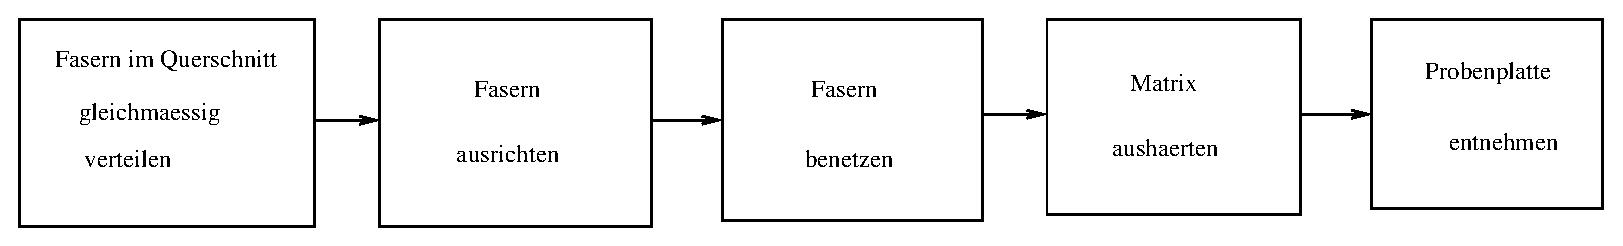
\includegraphics[width=14cm]{bilder/prozess.eps}
\hfill
\mbox

\vspace{1cm}
%
Beispiel f"ur einen Prozessablauf.

\subsection{Abbildung als Gleitobjekt}

Das ist "ahnlich wie bei den Tabellen.
\begin{figure}[!htb]
\includegraphics[height=7cm]{bilder/expo1.eps}
\caption{Die Exponentialverteilung}\label{fig:expo}
\end{figure}
